% app_c_t2.tex -- Appendix C: T2 audit details (27-task table, power arithmetic, proofs).
% Content moved verbatim from 04_t2_source_equiv.tex.

\section{Source Equivalence: Full Tables, Power Arithmetic, and Proofs}
\label{app:t2}

\subsection{Per-task source-equivalence table}
\label{app:t2-table}

% TABLE-t2: source equivalence. Source: tables/t2_source_equivalence.csv
\begin{table}[!htbp]
\centering
% TABLE-t2: per-task sigma_init, sigma_order, ratio, F and bootstrap CIs, band containment
% (source tables/t2_source_equivalence.csv)
\caption{\textbf{Source equivalence on the S\&N 1B arms.} Per-task ratio
$\sigma_{\mathrm{init}}/\sigma_{\mathrm{order}}$ --- below $1$ means the order arm is the
noisier one (e.g.\ \texttt{mbpp}: $0.0088/0.0133 = 0.66$) --- with F and bootstrap CIs (all 95\%), for 9 primary-like
and 18 bpb tasks, plus the F interval at the Bonferroni level ($\alpha = 0.05/27$;
conservative here, since 8 task identities appear in both panels). No task's analytic F
interval fits inside
the $2\times$ equivalence band ($0/27$; under the bootstrap intervals $2/27$ fit:
\texttt{winogrande} primary and \texttt{minerva\_math\_geometry} bpb); the two tasks whose uncorrected F CIs exclude 1 do so in opposite directions, and
neither survives multiplicity control (HellaSwag's bootstrap CI includes 1 as well).}
\label{tab:t2}
\scriptsize
\setlength{\tabcolsep}{3pt}
\begin{tabular}{@{}lcccccc@{}}
\toprule
task & $\hat\sigma_{\mathrm{init}}$ & $\hat\sigma_{\mathrm{order}}$ & ratio &
F CI & bootstrap CI & F CI (Bonf.) \\
\midrule
\multicolumn{7}{l}{\emph{primary-like accuracy tasks}}\\
\midrule
\texttt{hellaswag} & 0.00428 & 0.0124 & 0.35 & [0.17, 0.70] & [0.15, 1.26] & [0.10, 1.14] \\
\texttt{socialiqa} & 0.0123 & 0.0188 & 0.65 & [0.31, 1.32] & [0.37, 1.19] & [0.19, 2.11] \\
\texttt{mmlu} & 0.00401 & 0.00543 & 0.74 & [0.35, 1.50] & [0.43, 1.26] & [0.21, 2.41] \\
\texttt{arc\_challenge} & 0.0181 & 0.0241 & 0.75 & [0.36, 1.52] & [0.43, 1.75] & [0.22, 2.44] \\
\texttt{csqa} & 0.0125 & 0.0159 & 0.79 & [0.38, 1.59] & [0.29, 1.75] & [0.23, 2.57] \\
\texttt{winogrande} & 0.0129 & 0.0145 & 0.89 & [0.42, 1.79] & [0.51, 1.59] & [0.26, 2.89] \\
\texttt{arc\_easy} & 0.00869 & 0.00852 & 1.02 & [0.49, 2.07] & [0.64, 4.42] & [0.29, 3.32] \\
\texttt{piqa} & 0.00669 & 0.00641 & 1.04 & [0.50, 2.11] & [0.48, 3.03] & [0.30, 3.38] \\
\texttt{copycolors} & 0.127 & 0.107 & 1.18 & [0.57, 2.39] & [0.70, 2.24] & [0.34, 3.84] \\
\midrule
\multicolumn{7}{l}{\emph{bits-per-byte tasks}}\\
\midrule
\texttt{mbpp} & 0.00879 & 0.0133 & 0.66 & [0.32, 1.33] & [0.33, 1.39] & [0.19, 2.15] \\
\texttt{socialiqa} & 0.00817 & 0.0110 & 0.74 & [0.36, 1.51] & [0.47, 1.26] & [0.21, 2.41] \\
\texttt{minerva\_math\_counting\_and\_probability} & 0.00504 & 0.00585 & 0.86 & [0.41, 1.74] & [0.43, 1.90] & [0.25, 2.80] \\
\texttt{humaneval} & 0.0296 & 0.0343 & 0.86 & [0.41, 1.75] & [0.40, 1.68] & [0.25, 2.80] \\
\texttt{minerva\_math\_geometry} & 0.00521 & 0.00586 & 0.89 & [0.43, 1.80] & [0.52, 1.96] & [0.26, 2.89] \\
\texttt{arc\_challenge} & 0.00621 & 0.00688 & 0.90 & [0.43, 1.83] & [0.47, 2.22] & [0.26, 2.93] \\
\texttt{minerva\_math\_precalculus} & 0.00565 & 0.00607 & 0.93 & [0.45, 1.89] & [0.26, 2.67] & [0.27, 3.02] \\
\texttt{minerva\_math\_prealgebra} & 0.00416 & 0.00387 & 1.08 & [0.52, 2.18] & [0.36, 1.97] & [0.31, 3.51] \\
\texttt{piqa} & 0.00418 & 0.00362 & 1.16 & [0.55, 2.34] & [0.37, 2.52] & [0.33, 3.77] \\
\texttt{minerva\_math\_number\_theory} & 0.00345 & 0.00292 & 1.18 & [0.57, 2.40] & [0.35, 2.43] & [0.34, 3.84] \\
\texttt{csqa} & 0.0133 & 0.0109 & 1.22 & [0.58, 2.47] & [0.58, 3.97] & [0.35, 3.97] \\
\texttt{copycolors} & 0.0786 & 0.0632 & 1.24 & [0.60, 2.52] & [0.54, 2.35] & [0.36, 4.03] \\
\texttt{minerva\_math\_intermediate\_algebra} & 0.00526 & 0.00410 & 1.28 & [0.61, 2.60] & [0.62, 4.26] & [0.37, 4.16] \\
\texttt{gsm8k} & 0.0123 & 0.00904 & 1.36 & [0.65, 2.75] & [0.78, 3.01] & [0.39, 4.42] \\
\texttt{minerva\_math\_algebra} & 0.00484 & 0.00353 & 1.37 & [0.66, 2.78] & [0.62, 3.41] & [0.40, 4.46] \\
\texttt{arc\_easy} & 0.0152 & 0.0106 & 1.43 & [0.69, 2.91] & [0.67, 4.05] & [0.41, 4.65] \\
\texttt{hellaswag} & 0.00399 & 0.00213 & 1.88 & [0.90, 3.80] & [1.02, 3.25] & [0.54, 6.11] \\
\texttt{winogrande} & 0.0232 & 0.00982 & 2.36 & [1.13, 4.79] & [1.49, 4.52] & [0.68, 7.68] \\
\bottomrule
\end{tabular}
\end{table}

Setup: for each task we compute the within-arm relative SDs $\sigma_{\mathrm{init}}$ and
$\sigma_{\mathrm{order}}$ of final scores (mean of each run's last 3 checkpoints, arms truncated
to a common grid; Appendix~\ref{app:setup}), on 9 primary-like accuracy tasks and 18
bits-per-byte tasks. We assess source equivalence against a $[0.5, 2]$ band on the ratio
$\sigma_{\mathrm{init}}/\sigma_{\mathrm{order}}$ (a conventional factor-of-two
criterion) and report both F-distribution confidence
intervals (df 9 and 8) and run-level bootstrap intervals (2{,}000 resamples; percentile
bootstrap intervals on a variance ratio are known to under-cover at these arm sizes, so the
bootstrap containment counts are optimistic and the F intervals remain the primary
instrument). We report band
containment; we never read ``not significant'' as ``equivalent''.

\subsection{What it would take: the power arithmetic}
\label{app:t2-power}

% TABLE-t2power: n vs CI span vs pass probability. Source: VENUE-REASSESS.md N4 (lines 330-341)
% and GPU-SEGMENT-DECISION.md lines 59-65.
\begin{table}[!htbp]
\centering
% TABLE-t2power: n per arm, F_0.975 CI span, acceptance window, pass probability under true
% ratio = 1 (sources: GPU-SEGMENT-DECISION.md lines 59-65; VENUE-REASSESS.md lines 330-341)
\caption{\textbf{What it would take to decide source equivalence.} Half-width of the 95\%
F interval on the variance ratio (a pure function of degrees of freedom), the window of point estimates that
would land inside the $[0.5,2]$ band, and the probability of passing when the true ratio is 1.
The richest public arms ($n = 10$ vs.\ $9$) cannot pass; $n \ge 31$ per arm is needed for a 92\%
pass probability.}
\label{tab:t2power}
\footnotesize
\begin{tabular}{@{}cccc@{}}
\toprule
$n$ per arm & F-interval half-width (variance ratio) & acceptance window for $\hat r$ & pass prob.\ if true ratio $= 1$ \\
\midrule
3  & $39.0\times$ & none (span $>$ band) & 0\% \\
6  & $7.15\times$ & none & 0\% \\
8  & $4.99\times$ & none & 0\% \\
10 & $4.03\times$ & none & 0\% \\
10 vs.\ 9 (S\&N arms) & $4.23\times$ & none & 0\% \\
11 & $3.72\times$ & $[0.964, 1.037]$ & 9.0\% \\
16 & $2.86\times$ & $[0.846, 1.182]$ & 47.5\% \\
21 & $2.46\times$ & $[0.785, 1.274]$ & 71.3\% \\
31 & $2.07\times$ & $[0.720, 1.389]$ & 92.3\% \\
\bottomrule
\end{tabular}
\end{table}

The half-width of a variance-ratio CI is a pure function
of degrees of freedom, $F_{0.975}(\nu,\nu)$. With $n = 3$ per arm the interval's half-width is
$39\times$; $n = 6$ gives $7.15\times$; $n = 8$ gives $4.99\times$; even $n = 10$ gives
$4.03\times$, still wider than the $4\times$ band. The S\&N arms (df 9/8, half-width $4.23\times$)
are already the best the public record offers. Computing the pass probability under a true ratio
of exactly 1 sharpens the point: $n = 11$ per arm, the first size at which the band is
geometrically reachable, passes only $9\%$ of the time; $n = 16$ passes $47.5\%$; $n = 21$
passes $71\%$; only $n \ge 31$ per arm passes $92\%$ (Table~\ref{tab:t2power}).

\subsection{The non-identifiability remark: statement and proof}
\label{app:t2-proof}

Remark~\ref{prop:t2-nonid} is stated in the main text
(Section~\ref{sec:t2}, with its all-arm-sizes corollary in prose there); we prove it here. In part (i), the explicit binary example has
both arms equal to the same two-point law; the ratio $\sigma_{\mathrm{all}}^2/\sigma_i^2$ is
$1$, $2$, or $9$ depending on the unseen corner cell.

\emph{Remark (sharp but vacuous bounds).} Given the arm laws alone and scores in an interval of
width $B$, $\sigma_{\mathrm{all}}^2 \in [0, B^2/4]$, both endpoints attained (a constant score
gives the lower end; Popoviciu's inequality the upper, attained by a two-point law on the
boundary; $B{=}1$ for accuracy-like metrics, while bpb is unbounded above). In SD units the
identified interval for $\rho$ spans $[0, 3.9]$--$[0, 125]$ across primary tasks and
$[0, \infty)$ for all bpb tasks: the bounds certify nothing a practitioner could use, so we
report them only here.

\begin{proof}[Proof of Remark~\ref{prop:t2-nonid} (sketch)]
The arms pin down the laws of $a(I)$ and $b(D)$ and nothing else: under $I \perp D$ with
continuous sources the two arm lines have product measure zero, so the law of
$T = f(I,D)$ is unconstrained beyond the support. For (i), $c \equiv 0$ gives additivity,
while $c = -b$ off the order line gives $T = \mu + a(I)$, i.e.\
$\sigma_{\mathrm{all}}^2 = \sigma_i^2$; the binary example enumerates its four cells
directly. For (ii), with both covariances zero,
$\sigma_{\mathrm{all}}^2 = \sigma_i^2 + \sigma_o^2 + \mathrm{Var}(c) \ge
\sigma_i^2 + \sigma_o^2$, sharp at $c \equiv 0$.
\end{proof}

\paragraph{Which parametrization is in force, and what each estimator measures.}
The main text and the proof use the reference-cell parametrization: $c$ vanishes on both arm
lines, so each arm identifies its main-effect law exactly and
$\hat\sigma^2_{\mathrm{int}} = \hat\sigma^2_{\mathrm{bundled}} - \hat\sigma^2_{\mathrm{init}} -
\hat\sigma^2_{\mathrm{order}}$ (Appendix~\ref{app:crossed}) is an interaction contrast: it prices
$\mathrm{Var}(c)$ up to the latent--interaction covariances
$2\mathrm{Cov}(a,c)+2\mathrm{Cov}(b,c)$, which the arm-line constraints do not remove;
Appendix~\ref{app:crossed} finds it consistent with zero on all six tasks under either
reading.
Under the alternative sum-to-zero parametrization each arm's law already carries its
interaction slice --- the init arm at $d_0$ has variance $\mathrm{Var}(a(I) + c(I, d_0))$ ---
and the same non-identifiability conclusion holds, with the ``additivity factor'' then reading
$\sqrt{(\sigma_i^2 + \sigma_o^2 + \text{the arm-line interaction slices})}\,/\,\sigma_i$-like
quantities; the numerical factor in the text ($1.62\times$) is computed on the S\&N arms under
the reference-cell reading, which is the reading on which the arms identify main effects.

The $0/27$ of Table~\ref{tab:t2} is thus a
precision statement about the richest public arms, not evidence about the ratio: no enlargement of the single-source arms can
decide whether an init-only floor is faithful. Source parity ($\sigma_i = \sigma_o$)
remains identifiable (that is what Table~\ref{tab:t2power} prices, $n \ge 31$ per arm), but
answering it would not settle the floor. What identifies $\sigma_{\mathrm{all}}$ is a design
change: a bundled arm, or a crossed init$\times$order design \citep{dodge2020finetuning}, not more
single-source runs.

\subsection{Two readings of the init-only understatement}
\label{app:t2-bundle}

A natural repair is to inflate the init-only floor by the factor
$\sqrt{\sigma_{\mathrm{init}}^2 + \sigma_{\mathrm{order}}^2}/\sigma_{\mathrm{init}}$, which on
these arms has median $1.62$ (IQR $1.40$--$1.68$) on primary tasks and $1.32$ (IQR
$1.25$--$1.50$) on bpb. This number is a \textbf{model-based sensitivity
estimate} that assumes the two sources add independently with no interaction, not a measurement
of all-source noise, which these arms do not contain. Our own empirical cross-check lands lower:
DataDecide's 1B bundled-seed noise (which varies both sources jointly, on a different corpus and
architecture) sits at a median $1.06\times$ the S\&N init-only $\sigma$ ($1.19\times$ after
correcting the 3-seed SD's $c_4$ bias), though its own 95\% interval spans ${\sim}6\times$ at
df $= 2$. The point estimates do not establish per-task dominance after multiplicity control
(Section~\ref{sec:t2}); what removes the single-source floor as a task-level safe
surrogate for all-source noise is structural (Remark~\ref{prop:t2-nonid}). Whether such a floor understates or overstates the all-source noise on any
given task is not identifiable from these arms at any arm size
(Remark~\ref{prop:t2-nonid}); treating it as a precise community threshold is therefore
unfalsifiable as stated, not merely imprecise.

% TABLE-t2bundle: side-by-side presentation of 1.06/1.19 vs 1.62. Source:
% tables/t2_dd1b_vs_sn_bundle.csv + VENUE-REASSESS.md lines 222-226.
\begin{table}[!htbp]
\centering
% TABLE-t2bundle: model-based inflation vs empirical cross-check (source
% tables/t2_dd1b_vs_sn_bundle.csv; c4-corrected row per VENUE-REASSESS.md lines 222-226)
\caption{\textbf{Two readings of the init-only understatement.} Model-based sensitivity factor
$\sqrt{\sigma_i^2+\sigma_o^2}/\sigma_i$ (median $1.62$ primary / $1.32$ bpb, assumes independent
additive sources) against the empirical cross-check, DataDecide-1B bundled-seed $\hat\sigma$
over S\&N $\sigma_{\mathrm{init}}$ (median $1.06$; $1.19$ after $c_4$ correction, on df $= 2$).
We report the $1.62$ factor only as a sensitivity result under the additivity assumption; the
empirical check is compatible with it at current power but cannot confirm it.}
\label{tab:t2bundle}
\footnotesize
\begin{tabular}{@{}lcc@{}}
\toprule
quantity & median & spread \\
\midrule
\multicolumn{3}{l}{\emph{Model-based sensitivity factor $\sqrt{\sigma_i^2+\sigma_o^2}/\sigma_i$
(S\&N arms, per task)}}\\
\quad primary-like tasks (9) & $1.62$ & IQR $1.40$--$1.68$ \\
\quad bits-per-byte tasks (18) & $1.32$ & IQR $1.25$--$1.50$ \\
\midrule
\multicolumn{3}{l}{\emph{Empirical cross-check: DataDecide-1B bundled-seed $\hat\sigma$ /
S\&N $\sigma_{\mathrm{init}}$ (8 shared tasks)}}\\
\quad as measured & $1.06$ & IQR $0.92$--$1.19$ \\
\quad after $c_4$ bias correction & $1.19$ & df $= 2$; own 95\% interval spans ${\sim}6\times$ \\
\bottomrule
\end{tabular}
\end{table}

% FIG-F3 lives in this appendix since revision-3 batch 3 (page gate); its content is tab:t2.
\begin{figure}[!tbp]
\centering
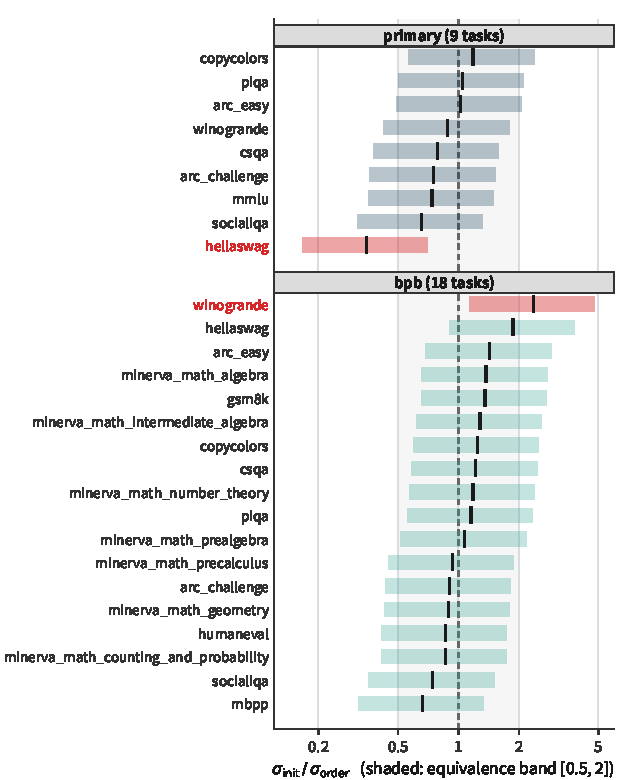
\includegraphics[width=0.76\linewidth]{figures/appc_forest.pdf}
\caption{\textbf{Source equivalence, task by task.} Per-task
$\sigma_{\mathrm{init}}/\sigma_{\mathrm{order}}$ with CIs vs.\ the
$[0.5, 2]$ band (shaded): no CI fits inside; the two tasks excluding 1 do so in opposite
directions, and neither survives Bonferroni control (Table~\ref{tab:t2}).}
\label{fig:t2}
\end{figure}

% FIG-t2plane: component view of fig:t2 (added 2026-09-03, revision-11 addendum).
\begin{figure}[!tbp]
\centering
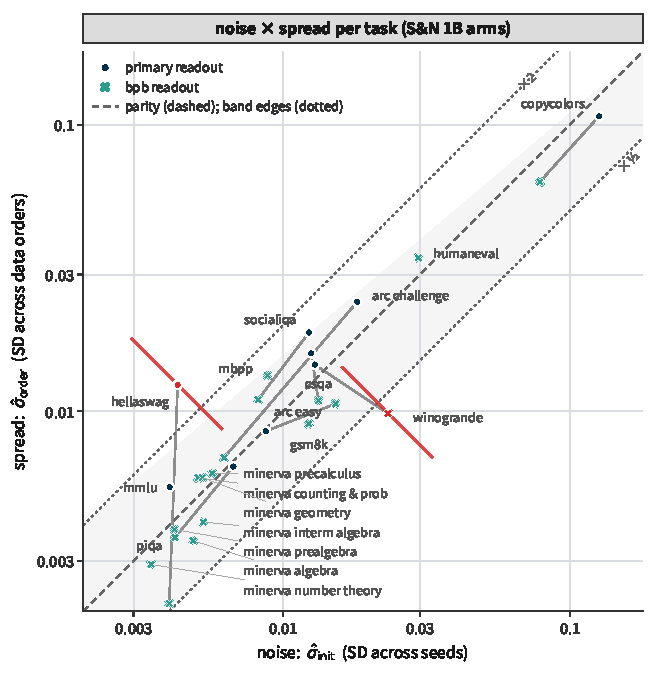
\includegraphics[width=0.80\linewidth]{figures/appc_noise_spread.pdf}
\caption{\textbf{The source-equivalence plane: noise against spread, task by task.}
Component view of Figure~\ref{fig:t2}: per-task $\hat\sigma_{\mathrm{init}}$ (SD across
seeds) against $\hat\sigma_{\mathrm{order}}$ (SD across data orders) on the S\&N 1B arms,
log--log with square decades, so parity is the 45$^\circ$ dashed diagonal and the
$[0.5, 2]$ equivalence band (shaded, dotted edges) is centred on it. Circles: primary
readout; crosses: bpb readout; grey segments join the eight task identities measured
under both. Point estimates mostly sit inside the band, while no 95\% interval fits
inside it (Figure~\ref{fig:t2}); only the two excluders carry their F interval here
(vermillion), each clearing parity in the opposite direction. Note the readout
dependence: \texttt{hellaswag} and \texttt{winogrande} each cross a band edge when
the readout changes (the former entering, the latter leaving), and the
\texttt{minerva\_math} family occupies the low-noise low-spread corner --- the
geometry behind the per-task ratios of Table~\ref{tab:t2}.}
\label{fig:t2plane}
\end{figure}
